\documentclass[tikz,border=0pt]{standalone}
\usepackage{amsmath, amssymb, bm}
\usetikzlibrary{positioning, arrows.meta, calc, fit, backgrounds}

\begin{document}
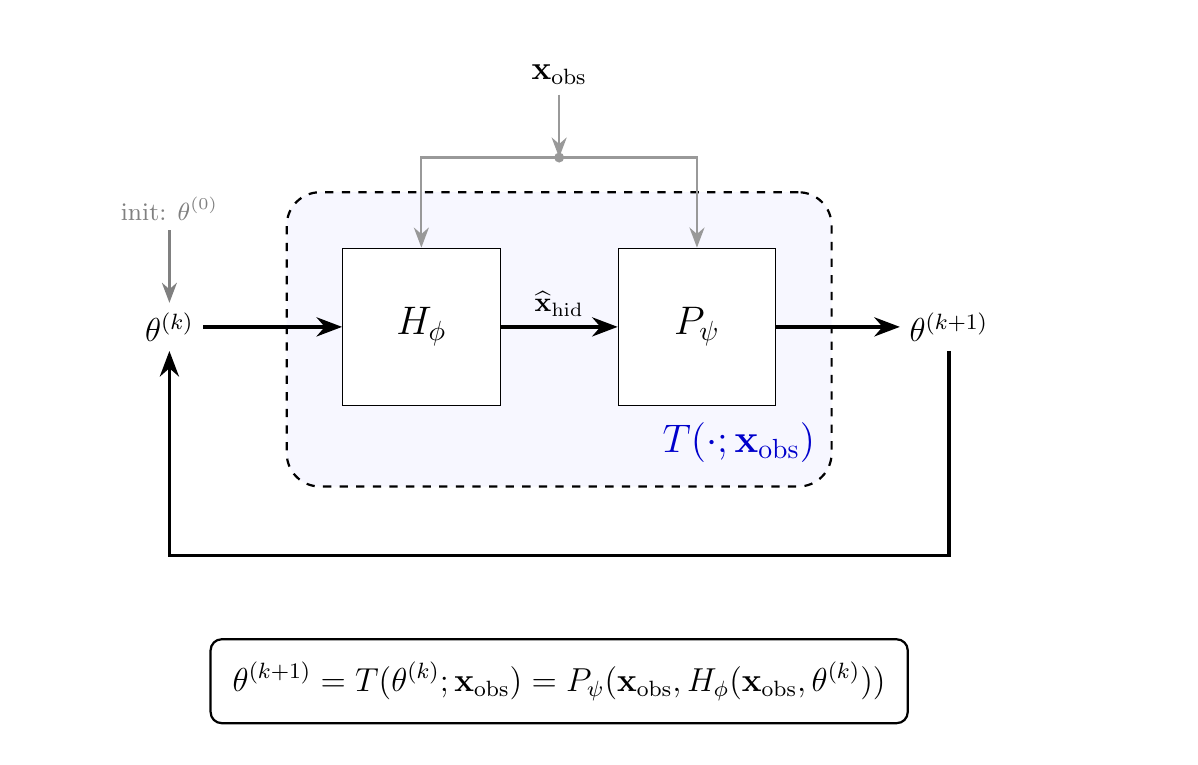
\begin{tikzpicture}[
    >={Stealth[scale=1.1]},
    netbox/.style={draw, rectangle, minimum width=2.0cm, minimum height=2.0cm, align=center, font=\Large, fill=white},
    txt/.style={align=center, font=\large},
    eqbox/.style={draw, rectangle, rounded corners, inner sep=8pt, font=\large, thick},
    uarrow/.style={->, thick, gray!80},
    mainarrow/.style={->, very thick, black}
]

% 두 그림의 크기와 기준점을 완벽히 일치시키는 강제 바운딩 박스
\useasboundingbox (-5.0, 3.8) rectangle (9.5, -5.2);

% Network Blocks
\node[netbox] (H_inf) at (0,0) {$H_\phi$};
\node[netbox] (P_inf) at (3.5,0) {$P_\psi$};

% T Operator Box
\begin{scope}[on background layer]
    \node (dummy_bottom) at (3.5, -1.2) {}; 
    \node[draw, rounded corners=12pt, dashed, thick, inner sep=20pt, fit=(H_inf) (P_inf) (dummy_bottom), fill=blue!3] (Tbox) {};
    \node[font=\Large\bfseries, text=blue!80!black, anchor=south east, xshift=-0.1cm, yshift=0.2cm] at (Tbox.south east) {$T(\cdot; \mathbf{x}_\mathrm{obs})$};
\end{scope}

% Dynamic Variables
\node[txt] (theta_in) at (-3.2, 0) {$\theta^{(k)}$};
\node[txt, font=\small, text=gray] (init) at (-3.2, 1.5) {init: $\theta^{(0)}$};
\node[txt] (theta_out) at (6.7, 0) {$\theta^{(k+1)}$};

% Global Parameter (u)
\node[txt] (u_input) at (1.75, 3.2) {$\mathbf{x}_\mathrm{obs}$};
\draw[uarrow] (u_input.south) -- ++(0,-0.8) coordinate (u_split);
\draw[uarrow] (u_split) -| (H_inf.north);
\draw[uarrow] (u_split) -| (P_inf.north);
\fill[gray!80] (u_split) circle (1.8pt);

% Main Flow
\draw[->, gray, thick] (init) -- (theta_in);
\draw[mainarrow] (theta_in) -- (H_inf.west);
\draw[mainarrow] (H_inf.east) -- (P_inf.west) node[midway, above] {$\widehat{\mathbf{x}}_{\mathrm{hid}}$};
\draw[mainarrow] (P_inf.east) -- (theta_out.west);

% Feedback Loop
\draw[mainarrow] (theta_out.south) -- ++(0,-2.6) coordinate (loop_right) -- (loop_right -| theta_in.south) coordinate (loop_left) -- (theta_in.south);

% Equation Box
\node[eqbox] (eq) at (1.75, -4.5) {
    $\displaystyle \theta^{(k+1)} = T(\theta^{(k)}; \mathbf{x}_\mathrm{obs}) = P_\psi(\mathbf{x}_\mathrm{obs}, H_\phi(\mathbf{x}_\mathrm{obs}, \theta^{(k)}))$
};

\end{tikzpicture}
\end{document}